\section{Deformation quantization and algebraic index}\label{sec:dqai}

Recall that we discussed in the \nameref{subsec:heat}, the family $\lcb I[L]\rcb_{L>0}$ satisfies the homotopy RG.
\bea
\tikzset{every picture/.style={line width=0.75pt}} %set default line width to 0.75pt
\begin{tikzpicture}[x=0.75pt,y=0.75pt,yscale=-1,xscale=1]
%uncomment if require: \path (0,300); %set diagram left start at 0, and has height of 300
%Straight Lines [id:da977711475048066] 
\draw    (10.5,100.67) -- (237.5,100.67) ;
\draw [shift={(240.5,100.67)}, rotate = 180] [fill={rgb, 255:red, 0; green, 0; blue, 0 }  ][line width=0.08]  [draw opacity=0] (10.72,-5.15) -- (0,0) -- (10.72,5.15) -- (7.12,0) -- cycle    ;

% Text Node
\draw (4,78.23) node [anchor=north west][inner sep=0.75pt]    {$0$};
% Text Node
\draw (3.12,96) node [anchor=north west][inner sep=0.75pt]  [font=\normalsize,rotate=-0.88]  {$\blt$};
% Text Node
\draw (58,96) node [anchor=north west][inner sep=0.75pt]  [font=\normalsize,rotate=-0.88]  {$\blt$};
% Text Node
\draw (166.12,96) node [anchor=north west][inner sep=0.75pt]  [font=\normalsize,rotate=-0.88]  {$\blt$};
% Text Node
\draw (58,77.23) node [anchor=north west][inner sep=0.75pt]    {$L_{1}$};
% Text Node
\draw (165.5,76.23) node [anchor=north west][inner sep=0.75pt]    {$L_{2}$};
% Text Node
\draw (245.5,93.07) node [anchor=north west][inner sep=0.75pt]    {$L$};
% Text Node
\draw (40.5,108.07) node [anchor=north west][inner sep=0.75pt]    {$I[L_{1}]$};
% Text Node
\draw (152.5,108.07) node [anchor=north west][inner sep=0.75pt]    {$I[L_{2}]$};
% Text Node
\draw (100,106.57) node [anchor=north west][inner sep=0.75pt]    {$\overset{\text{HRG}}{\leadsto}$};
\end{tikzpicture}
\eea
At $L\to 0$, we use the counter-term method to reduce the ill-defined theory with UV divergence to a well-defined effective theory.
At each $L>0$, we have a well-defined effective BV operator $\Delta_L$, which is a contraction with the smooth kernel $K_L$ representing $e^{-L\lsb Q,Q^\dagger\rsb}$. This leads to the effective DGBV, $\lb \cO(\cE), Q, \Delta_L\rb$, in which the corresponding $I[L]$ solves the QME.

Let $\bH=\lcb \left. \varphi\in\cE\ \right|\ \lsb Q,Q^\dagger\rsb\varphi=0\rcb\ = 
\lcb \left. \varphi\in\cE\ \right|\  Q\varphi=Q^\dagger\varphi=0\rcb\ \simeq H^\blt\lb \cE,Q\rb$. $\bH$ is called the space of \textbf{harmonics} (or the \textbf{zero modes}), which is a finite-dimensional space (by Hodge theory).
Then we have
\bea
\begin{tikzcd}
\infty-\text{dimensional } (-1)-\text{symplectic geometry } (\cE,Q,\omega)  \ar[d, "L\to\infty"] \\
\text{finite-dimensional } (-1)-\text{symplectic geometry } (\bH,\omega_H
=\left. \omega \right|_{\bH})
\end{tikzcd}
\eea

The BV operator $\Delta_H$ associated to $\omega_H^{-1}$ is $\Delta_H=\Delta_\infty$. On the complete story of BV quantization, we have
\bea
\tikzset{every picture/.style={line width=0.75pt}} %set default line width to 0.75pt
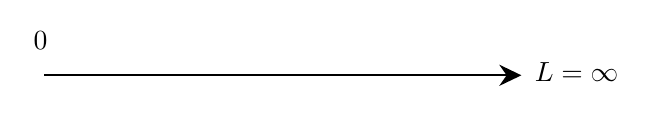
\begin{tikzpicture}[x=0.75pt,y=0.75pt,yscale=-1,xscale=1]
%uncomment if require: \path (0,300); %set diagram left start at 0, and has height of 300
%Straight Lines [id:da977711475048066] 
\draw    (10.5,100.67) -- (237.5,100.67) ;
\draw [shift={(240.5,100.67)}, rotate = 180] [fill={rgb, 255:red, 0; green, 0; blue, 0 }  ][line width=0.08]  [draw opacity=0] (10.72,-5.15) -- (0,0) -- (10.72,5.15) -- (7.12,0) -- cycle    ;

% Text Node
\draw (4,78.23) node [anchor=north west][inner sep=0.75pt]    {$0$};
% Text Node
\draw (3.12,96) node [anchor=north west][inner sep=0.75pt]  [font=\normalsize,rotate=-0.88]  {$\blt$};

% Text Node
\draw (245.5,93.07) node [anchor=north west][inner sep=0.75pt]    {$L=\infty$};
\end{tikzpicture}
\eea
where $I[\infty]$ solves the QME for $\lb \cO(\bH),\Delta_H\rb$. This is an interesting point where we will find some finite-dimensional geometric data, leading to the index theory.

Our next goal is to use the method we have discussed so far to do \emph{geometry and topology}.
We will explain two main examples:
\bi[(1)]
\item 1d example: topological quantum mechanics and algebraic index.
\textsc{References}: \cite{Grady:2015ica,Gui:2019ldd}.

\item 2d example: chiral CFT and chiral index. 
\textsc{References}: \cite{Li:2016gcb,Gui:2021dci}.
\ei

\subsection*{Deformation quantization}
\begin{defn}
A \textbf{Poisson manifold} is a pair $\lb X,P\rb$, where $X$ is a smooth manifold, and $P\in \Gamma(X, \asym^2 TX)$ satisfying $\lcb P,P\rcb_{\text{SN}}=0$.
\end{defn}
$\lcb -,-\rcb_{\text{SN}}$ is the \emph{Schouten-Nijenhuis bracket}. $P$ is called the \textbf{Poisson tensor/bi-vector}. In local coordinates, we can write 
\bea P=\sum_{i,j} P^{ij}(x)\p_i \wedge \p_j.\eea
It defines a \emph{Poisson bracket} $\lcb-,-\rcb_P$ on $C^\infty(x)$:
\bea \lcb f,g\rcb_P \coloneqq \sum_{i,j} P^{ij}\p_i f \p_j g,\quad \forall f,g\in C^\infty(x).\eea
Here $\lcb P,P\rcb_{\text{SN}}=0$ implies that $\lcb-,-\rcb_P$ satisfies Jacobi identity. Hence $\lcb-,-\rcb_P$ naturally defines the Poisson algebra $\lb C^\infty(x), \lcb-,-\rcb_P\rb$.

\begin{eg}
Let $(X,\omega)$ be a symplectic manifold, where $\omega= \hf\sum_{i,j} \omega_{ij} dx^i \wedge dx^j$ is a symplectic 2-form. Let 
$P=\omega^{-1}=\hf \sum_{i,j} \omega^{ij} \p_i \wedge \p_j$,
where $(\omega^{ij})$ is the inverse of $(\omega_{ij})$. Then $d\omega=0 \LRA \lcb P,P\rcb_{\text{SN}}=0$. Hence $(X,\omega^{-1})$ is a Poisson manifold.
\end{eg}

\paragraph{Deformation quantization.}
This method was developed in the series of papers by Bayen, Flato, Fronsdal, Lichnerowicz, Sternheimer (BFFLS) \cite{bayen1977quantum,BAYEN197861,BAYEN1978111}. The space of the real-valued (or complex-valued) functions on a phase space admits
two algebraic structures: a structure of \emph{associative algebra} given by the usual product of
functions and a structure of Lie algebra given by the \emph{Poisson bracket}. The study of the
properties of the deformations (in a suitable sense) of these two structures gives a new
invariant approach for Quantum Mechanics (QM) and Quantum Field Theory (QFT).
\bea
\begin{tikzcd}
\text{Poisson Lie algebra}
\arrow[r, bend left, "\text{quantization}"] & \arrow[l, bend left, "\hbar\to 0"] \text{Associative algebra} 
\end{tikzcd}\eea
This is essentially the way of quantization in quantum mechanics, in which a function $f$ on the classical phase space is quantized to an operator $\widehat{f}$.

\begin{defn}
A \textbf{star-product} on a Poisson manifold $(X,P)$ is a $\bR\llb \hbar\rrb$-bilinear map
\bea C^\infty(x)\llb \hbar\rrb \times C^\infty(x)\llb \hbar\rrb \to C^\infty(x)\llb \hbar\rrb, \qquad 
f \times g \mapsto f\ast g=\sum_{k\geq 0} \hbar^k c_k\lb f,g\rb 
\eea
such that
\bi[(1)]
\item $\ast$ is associative: $\lb f\ast g\rb \ast h=f\ast \lb g\ast h\rb$,
\item $f\ast g= fg+\cO(\hbar), \quad \forall f,g\in C^\infty(x)$,
\item $\ast$ is non-commutative: $\hf \lb f\ast g-g\ast f\rb=\hbar\lcb f,g\rcb+\cO(\hbar^2), \quad \forall f,g\in C^\infty(x)$,
\item $c_k: C^\infty(x)\times C^\infty(x)\to C^\infty(x)$ is a bidifferential operator. 
\ei
Then $\lb C^\infty(x)\llb\hbar\rrb, \ast\rb$ is called a \textbf{deformation quantization} of $\lb X,P\rb$.
\end{defn}

The deformation quantization is purely algebraic; no Hilbert space is involved.
The \emph{existence} of deformation quantization is highly nontrivial. In particular, the existence of formal star product on symplectic manifolds was proved by de Wilde-LeConte \cite{de1983existence} and Fedosov \cite{fedosov1994simple}.
More generally, Kontsevich \cite{Kontsevich:1997vb} gave the complete solution for general Poisson manifold. 

\begin{eg}[Moyal-Weyl product]
Let $X$ be a phase space, $\bR^{2n}$, with a symplectic form $\omega=\hf \sum_{i,j} \omega_{ij} dx^i \wedge dx^j$ where $\omega_{ij}$ is a constant. The Poisson tensor is $P=\hf \sum_{i,j} \omega^{ij} \p_i\wedge \p_j$. Given $f(x),g(x)\in C^\infty\lb \bR^{2n}\rb$, define the Moyal-Weyl product $\ast$ by
\bea
(f\ast g)(x)=\left. \exp{\lb \frac{\hbar}{2} \sum_{i,j} \omega^{ij} \frac{\p}{\p y^i}\frac{\p}{\p z^j}\rb}\right|_{y=z=x} f(y) g(z)
\eea
or pictorially,\\
\bea 
    \begin{fmffile}{fmw}
    \begin{tabular}{c}
        \begin{fmfgraph*}(150,50)
                \fmfleft{i1,i2}
                \fmfright{o1,o2}
    
                \fmf{plain,tension=4}{i1,v1}
                \fmf{plain,tension=4}{i2,v1}
                \fmf{plain,tension=4}{v2,o1}
                \fmf{plain,tension=4}{v2,o2}
        
                \fmf{plain,left=1,tension=0.4,label=$\frac{\p}{\p x^i} \omega^{ij} \frac{\p}{\p x^j}$,label.side=left}{v1,v2}
                \fmf{plain,left=0.5,tension=0.8}{v1,v2}
                \fmf{phantom,right=0.2,tension=2,label=$\cdot$,label.side=left}{v1,v2}
                \fmf{phantom,right=0.5,tension=0.8,label=$\cdot$,label.side=left}{v1,v2}
                \fmf{phantom,right=0.8,tension=0.6,label=$\cdot$,label.side=left}{v1,v2}
                \fmf{plain,right=1,tension=0.4}{v1,v2}
                
                \fmfv{label=$f\ $,label.angle=180,decor.shape=circle,decor.filled=full,decor.size=2thick}{v1}
                \fmfv{label=$\ g$,label.angle=0,decor.shape=circle,decor.filled=full,decor.size=2thick}{v2}
        \end{fmfgraph*}
        \end{tabular}
    \end{fmffile}
\eea
Then $\ast$ defines a deformation quantization.
\end{eg}

\begin{rmk}
If $\omega^{ij}\neq$ constant, then the above formula does not work. 
\end{rmk}

For convenience, we can describe a formal version. Let $\lb V,\omega\rb$ be a linear symplectic space, where $V\cong \bR^{2n}$ and $\omega: \asym^2 V\to \bR$ is a symplectic pairing. Write 
\bea\widehat{\cO}(V)\coloneqq \widehat{\sym}(V^\vee)=\prod_{k\geq 0} \sym^k(V^\vee),\eea
where $V^\vee=\on{Hom}(V,\bR)$ is the linear dual of $V$. Then the Moyal-Weyl product defines an associative algebra $\lb \widehat{\cO}(V)\llb \hbar\rrb,\ast\rb$, called the (formal) Weyl algebra. On the other hand, let 
\bea\widehat{\Omega}^{-\blt}_{V}\coloneqq \widehat{\cO}(V) \otimes \asym^{-\blt}(V^\vee).
\eea
Here $\widehat{\Omega}^{-p}_{V}\coloneqq \widehat{\cO}(V) \otimes \asym^{p}(V^\vee)$ are the (formal) $p$-forms sitting in degree $-p$. Let $d_V: \widehat{\Omega}^{-p}_{V} \to \widehat{\Omega}^{-(p+1)}_{V}$ be de Rham differential. Let $\pi=\omega^{-1}\in\asym^2 V$ be the Poisson tensor and $\iota_\pi: \widehat{\Omega}^{-\blt}_{V}\to \widehat{\Omega}^{-(\blt-2)}_{V}$ be the contraction with $\pi$. Let $\Delta=\cL_\pi=\lsb d_V,\iota_\pi\rsb: \widehat{\Omega}^{-\blt}_{V}\to\widehat{\Omega}^{-(\blt-1)}_{V}$ be the Lie derivative. Thus $\lb \widehat{\Omega}^{-\blt}_{V},\Delta\rb$ defines a BV algebra. Geometrically, this leads to Koszul-Brylinski complex/homology. Physically, this is the effective geometry on \emph{zero modes} of topological quantum mechanics as we will see.

\subsection*{Fedosov quantization}
We will focus on \emph{symplectic manifolds} now. Fedosov \cite{fedosov1994simple} gave a simple and geometric construction of deformation quantization on symplectic cases. 
\begin{defn}
Let $(X,\omega)$ be a symplectic manifold.
We define the \textbf{Weyl bundle} 
\bea W(X)\coloneqq \prod_{k\geq 0}\sym^k\lb T^\ast X\rb\llb \hbar\rrb.\eea
So at each point $p\in X$, its fiber is
\bea \left. W(X)\right|_p= \widehat{\cO}\lb T_p X\rb\llb\hbar\rrb.\eea
\end{defn}
A local section of $W(X)$ is 
\bea \sigma(x,y)=\sum_{k,l\geq 0}\hbar^k a_{k,i_1\cdots i_l}(x) y^{i_1}\cdots y^{i_l},\eea
where $\lcb x\rcb$ are the base coordinates and $\lcb y\rcb$ are the fiber coordinates; $a_{k,i_1\cdots i_l}(x)$ are smooth functions.
Since $\lb T_p X, \left.\omega\right|_{T_p X}\rb$ is linear symplectic, we have a fiberwise Moyal-Weyl product, still denoted by $\ast$. Thus $\lb W(X),\ast\rb$ defines the $\infty$-dimensional bundle of algebras.

Let $\nabla$ be a connection on $TX$ which is torsion-free and compatible with $\omega$ ($\nabla \omega=0$). Such connection is called a \textbf{symplectic connection} (which always exist and is not unique). $\nabla$ induces a connection on all tensors. In particular, it defines a connection on $W(X)$, still denoted by $\nabla$. Its curvature is
\bea \nabla^2 \sigma=\frac{1}{\hbar}\lsb R_\nabla, \sigma\rsb_\ast, \quad \forall \sigma\in \Gamma(X,W(X))\eea
where $R_\nabla=\frac{1}{4}R_{ijkl} y^i y^j dx^k \wedge dx^l \in \Omega^2(X,W(X))$ is a 2-form valued in the Weyl algebra; $R_{ijkl}=\omega_{im}R^m{}_{jkl}$ is a curvature form contracted with the symplectic pairing.

\paragraph{Fedosov's construction.}
Given a sequence of closed 2-forms $\lcb \omega_k\rcb_{k\geq 1}$ on $X$, there exists a unique (up to gauge) connection on $W(X)$ of the form $\nabla+\frac{1}{\hbar}\lsb \gamma,-\rsb_\ast, \gamma\in\Omega^1\lb X, W(X)\rb$, satisfying some initial conditions and the equation 
\bea \nabla\gamma+\frac{1}{2\hbar}\lsb \gamma,\gamma\rsb_\ast+R_\nabla=\omega_\hbar\qquad \text{(Fedosov equation)}\eea
where $\omega_\hbar=-\omega+ \sum_{k\geq 1}\hbar^k \omega_k$.

Let $D= \nabla+\frac{1}{\hbar}\lsb \gamma,-\rsb_\ast$. Then the Fedosov equation implies $D^2=\frac{1}{\hbar}\lsb\omega_\hbar,-\rsb_\ast=0$, where $\omega_\hbar$ is constant along each fiber, and thus a central term.
So we obtain a flat connection $D$ on $W(X)$. Let $W_D(X)\coloneqq \lcb \left.\sigma\in\Gamma(X,W(X))\ \right|\ D\sigma=0 \rcb$ be the space of flat sections. Then $\lb W_D(X),\ast\rb$ is an associative algebra.

Let $\sigma: W_D(X)\to C^\infty(X)\llb\hbar\rrb$ by sending $y\mapsto 0$ (\textbf{symbol map}). Then $\sigma$ is an isomorphism, and 
\bea f\ast g \mapsto \sigma\lb \sigma^{-1}\lb f\rb\ast \sigma^{-1}\lb g\rb\rb\eea
defines a deformation quantization. $\omega_\hbar$ is the corresponding \textbf{characteristic class} (or \textbf{moduli}).

\subsection*{Algebraic index theorem}
Given a deformation quantization $\lb C^\infty(X)\llb\hbar\rrb,\ast \rb$ on a symplectic manifold with characteristic class $\omega_\hbar$, there exists a unique \textbf{trace map}
\bea \Tr: C^\infty(X)\llb\hbar\rrb \to \bR\llb \hbar\rrb\eea
satisfying a normalization condition and the trace property:
\bea \Tr \lb f\ast g\rb=\Tr \lb g\ast f\rb.\eea
Then the index is obtained as the partition function of the theory, which can be formulated as 
\bea \on{Index}=\Tr(1)=\int_X e^{\omega_\hbar/\hbar} \widehat{A}(X),\eea
where $\widehat{A}(X)$ is the formal $\widehat{A}$-genus of $X$.
This is the simplest version of algebraic index theorem formulated by Fedosov and Nest-Tsygan as the algebraic analogue of Atiyah-Singer index theorem. 

We can similarly construct a \emph{deformation quantization} for $C^\infty\lb X,\on{End}(E)\rb\llb\hbar\rrb$ and construct the trace map, then we have $\Tr(1)=\int_X e^{\omega_\hbar/\hbar}\on{ch}(E) \widehat{A}(X)$.

\subsection*{Relation with QFT}
In supersymmetric (SUSY) QFT, \emph{localization} often appears:
\bea \int_\cE e^{iS/\hbar}= \int_M \lb -\rb,\eea
where $M\subset \cE$ is a finite-dimensional space describing some interesting moduli space.

In topological QM, we find
\bea \int_{\on{Map}(S^1,X)} e^{-S/\hbar}= \int_X \lb -\rb,\eea
where $\int_X$ indicates the localization to constant loops. The left-hand side of the equation is an analytic index; the right-hand side is a topological index.
In the next section, we would like to present a physics \emph{derivation} of the index theorem.

\begin{comment}
Geometrically, a loop space (circle) is mapped to a localized neighborhood of a point in $X$, where a localized effective theory exists.
\begin{figure}[!htpb]\centering 
\tikzset{every picture/.style={line width=0.75pt}} %set default line width to 0.75pt        

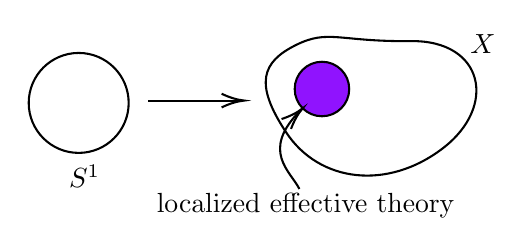
\begin{tikzpicture}[x=0.75pt,y=0.75pt,yscale=-1,xscale=1]
%uncomment if require: \path (0,300); %set diagram left start at 0, and has height of 300

%Shape: Ellipse [id:dp96215148925455] 
\draw   (18.33,67.88) .. controls (18.33,54.58) and (29.11,43.8) .. (42.41,43.8) .. controls (55.71,43.8) and (66.49,54.58) .. (66.49,67.88) .. controls (66.49,81.18) and (55.71,91.96) .. (42.41,91.96) .. controls (29.11,91.96) and (18.33,81.18) .. (18.33,67.88) -- cycle ;
%Straight Lines [id:da3304787521485182] 
\draw    (76.04,66.75) -- (120.21,66.75) ;
\draw [shift={(122.21,66.75)}, rotate = 180] [color={rgb, 255:red, 0; green, 0; blue, 0 }  ][line width=0.75]    (10.93,-3.29) .. controls (6.95,-1.4) and (3.31,-0.3) .. (0,0) .. controls (3.31,0.3) and (6.95,1.4) .. (10.93,3.29)   ;
%Shape: Polygon Curved [id:ds07244034873824146] 
\draw   (146.88,40.09) .. controls (162.8,32.13) and (167.58,38.5) .. (202.6,38.1) .. controls (237.62,37.7) and (244.39,69.54) .. (217.72,89.84) .. controls (191.06,110.13) and (158.42,106.15) .. (142.5,82.27) .. controls (126.58,58.39) and (130.96,48.05) .. (146.88,40.09) -- cycle ;
%Shape: Ellipse [id:dp8249251345393571] 
\draw  [fill={rgb, 255:red, 144; green, 19; blue, 254 }  ,fill opacity=1 ] (146.48,61.18) .. controls (146.48,53.93) and (152.36,48.05) .. (159.62,48.05) .. controls (166.87,48.05) and (172.75,53.93) .. (172.75,61.18) .. controls (172.75,68.43) and (166.87,74.31) .. (159.62,74.31) .. controls (152.36,74.31) and (146.48,68.43) .. (146.48,61.18) -- cycle ;
%Curve Lines [id:da6993644771515923] 
\draw    (148.74,109.34) .. controls (144.55,100.89) and (129.84,91.03) .. (149.11,71.66) ;
\draw [shift={(150.33,70.47)}, rotate = 136.29] [color={rgb, 255:red, 0; green, 0; blue, 0 }  ][line width=0.75]    (10.93,-3.29) .. controls (6.95,-1.4) and (3.31,-0.3) .. (0,0) .. controls (3.31,0.3) and (6.95,1.4) .. (10.93,3.29)   ;

% Text Node
\draw (36.29,96.06) node [anchor=north west][inner sep=0.75pt]    {$S^{1}$};
% Text Node
\draw (78.53,110) node [anchor=north west][inner sep=0.75pt]   [align=left] {localized effective theory};
% Text Node
\draw (229.63,33.68) node [anchor=north west][inner sep=0.75pt]    {$X$};


\end{tikzpicture}
\end{figure}

Locally, using Dolbeault coordinates, a loop space can be thought of as a standard phase space, $\bR^{2n}$. 
\begin{figure}[!htpb]\centering
\tikzset{every picture/.style={line width=0.75pt}} %set default line width to 0.75pt        

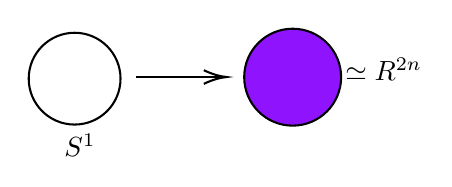
\begin{tikzpicture}[x=0.75pt,y=0.75pt,yscale=-1,xscale=1]
%uncomment if require: \path (0,300); %set diagram left start at 0, and has height of 300

%Shape: Ellipse [id:dp3832555122004915] 
\draw   (27.67,44.07) .. controls (27.67,31.85) and (37.57,21.95) .. (49.78,21.95) .. controls (62,21.95) and (71.9,31.85) .. (71.9,44.07) .. controls (71.9,56.28) and (62,66.18) .. (49.78,66.18) .. controls (37.57,66.18) and (27.67,56.28) .. (27.67,44.07) -- cycle ;
%Straight Lines [id:da9240446990399585] 
\draw    (79.34,43.28) -- (120.96,43.28) ;
\draw [shift={(122.96,43.28)}, rotate = 180] [color={rgb, 255:red, 0; green, 0; blue, 0 }  ][line width=0.75]    (10.93,-3.29) .. controls (6.95,-1.4) and (3.31,-0.3) .. (0,0) .. controls (3.31,0.3) and (6.95,1.4) .. (10.93,3.29)   ;
%Shape: Ellipse [id:dp2967020000357363] 
\draw  [fill={rgb, 255:red, 144; green, 19; blue, 254 }  ,fill opacity=1 ] (131.49,43.35) .. controls (131.49,30.45) and (141.94,20) .. (154.84,20) .. controls (167.73,20) and (178.19,30.45) .. (178.19,43.35) .. controls (178.19,56.24) and (167.73,66.7) .. (154.84,66.7) .. controls (141.94,66.7) and (131.49,56.24) .. (131.49,43.35) -- cycle ;

% Text Node
\draw (43.39,69.3) node [anchor=north west][inner sep=0.75pt]    {$S^{1}$};
% Text Node
\draw (178.79,32.74) node [anchor=north west][inner sep=0.75pt]    {$\simeq \mathbb{R}^{2n}$};

\end{tikzpicture}
\end{figure}
The loop spaces are then glued together on $X$ as a family of effective field theory. This can be done rigorously within the framework of effective BV quantization:
\begin{itemize}
    \item Effective action $\leadsto \gamma$,
    \item QME $\leadsto$ Fedosov equation,
    \item BV integral $\leadsto$ trace map,
    \item partition function $\leadsto$ algebraic index.
\end{itemize}
\end{comment}
